\documentclass[10pt]{article}
\usepackage[utf8]{inputenc}
\usepackage{url}
\usepackage{hyperref}
\usepackage{amsmath}
\usepackage{amsfonts}
\usepackage{amssymb}
\usepackage{graphicx}
\graphicspath{ {./images/} }
\usepackage{float}
\usepackage{lipsum}
\usepackage{sectsty}
\usepackage{tikz}
\sectionfont{\centering}
\usepackage{multicol}
\usepackage{xcolor}
\usepackage{natbib}
\usepackage{graphicx}
\usepackage{listings}
\usepackage{xcolor}
\usepackage{pgfplots}
\usepackage[font=small]{caption}
\addtolength{\abovecaptionskip}{-3mm}
\addtolength{\textfloatsep}{-5mm}
\setlength\columnsep{20pt}

\usepackage[a4paper,left=1.50cm, right=1.50cm, top=2cm, bottom=3cm]{geometry}


\author{}

\title{\Large{Design and Analysis of Algorithms Assignment - 2}}
\begin{document}
	\begin{center}
		{\Large \textbf{Design and Analysis of Algorithms Assignment - 2}}\\
		\vspace{1em}
		{\large Department of Information Technology}\\
		\vspace{1em}
		\large{Indian Institute of Information Technology - Allahabad, India}\\
		\vspace{1em}
		\large{Gitika Yadav \hspace{10em} Divyatez Singh \hspace{9em} Divyansh Rai}
		\large{IIT2019219 \hspace{10.5em} IIT2019220 \hspace{10.5em} IIT2019221}
		
		\vspace{2.5em}
	\end{center}
	
\begin{multicols*}{2}

    \textbf{\emph{{Abstract}: Given a positive integer namely n. The problem is to find out the sum of those n natural numbers, i.e, 1 + 2 + 3 + ..... + n. This paper discusses a Divide and Conquer algorithm-based solution for the given problem. This time complexity of this approach is measured to be O(N).}}\\
	
	\textbf{\emph{{Index Terms}: Arrays, Divide and Conquer, Recursion\\}}


\section*{INTRODUCTION}
 
We have been given a set (or array) of positive contiguous natural numbers. An array is a linear data structure which stores similar elements in contiguous memory locations. A Recursion method has been used on the array.

\paragraph{Divide and Conquer}
Divide and Conquer is a programming paradigm based on the concept of dividing then merging. A divide-and-conquer algorithm recursively breaks down a problem into two or more sub-problems (divide part), until these become simple enough to be solved directly (conquer part). The solutions to the sub-problems are then combined to give a solution to the original problem. The approach of divide and conquer generally follows three important aspects:
\begin{enumerate}
    \item\textbf{Divide:} This involves dividing the problem into some sub problem.
    \item\textbf{Conquer:} Sub problem by calling recursively until sub problem solved.
    \item\textbf{Combine:} The Sub problem Solved so that we will get find problem solution.Let us have a pictorial look of the image which makes the concept of Divide and Conquer Paradigm self explanatory.\\\\
\end{enumerate}

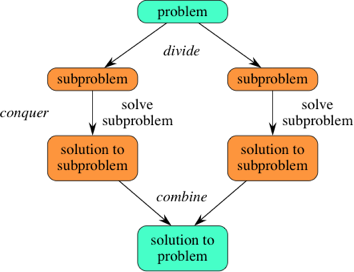
\includegraphics[width=\columnwidth, height=8cm]{dandc.png}\begin{center}\textbf{Figure 1:} Divide and Conquer\end{center}


\paragraph{Advantages of Divide and Conquer}
The Divide and Conquer technique generally has following mentioned advantages over Brute Force Algorithms.\\\\
\textbf{Time Efficiency} This approach reduces the running time of the algorithm because of its logarithmic nature. This is because the approach of Divide and Conquer keeps on dividing which makes it logarithmic in nature.\\\\
\textbf{Space Efficiency:} As no need to mention the algorithm,  but still, the space complexity also reduces up to a much extent due to the nature of dividing and then merging up.\\

\\This report further contains:
\begin{itemize}
\item 	Algorithm  Designs
\item 	Algorithm  Analysis
\item 	Experimental Study and Profiling
\item 	Conclusion
\item 	References
\item 	Appendix
\end{itemize}

\section*{ALGORITHM DESIGN}
A general problem based on the divide and conquer approach in which, we divided the problem into sub tasks and then make decisions while capturing the answer and merging. The data structure used in finding the sum of natural numbers are the standard and primary data structure of the computational domain. Following structures have been taken into account while making the code for the report.

\paragraph{Algorithmic Steps:}

Basically, the approach based on Divide and Conquer paradigm of finding the sum of natural numbers, generally has the steps defined in following algorithmic procedure, which have been implemented while solving the problem:
\begin{enumerate}

\item	Input a number upto which sum has to be considered using random number generator function.
\item	Store contiguous natural numbers starting from 1 to n in an array namely arr.
\item	Create a function sumArray, which takes input array and its size.
\item	sumArray implements base cases if applicable or divides array in two halves.
\item	Then the sum is calculated for the two halves and further recursively calling the function sumArray.
\item	Finally sum of both halves is returned.
\end{enumerate}

The above returned sum is the sum of n natural numbers.

\lstset { %
    language=C++,
    backgroundcolor=\color{black!5},
    basicstyle=\footnotesize,
}

\begin{lstlisting}
        
Int:
Function sumArray(Array, int size)
	if size == 0
	    return 0
	else if size ==1
	    return Array[0];
	
	int mid = size / 2
    int rsize = size - mid
    int lsum = sumArray(Array, mid)
    int rsum = sumArray(Array + mid, rsize)
    return lsum + rsum


Int:
Function main()
    int n
    print Enter a number
    Input n
    
    arr :array
    loop i=1 to n with i++
        arr[i-1] = i
    
    print The smallest distance is 
    print sumArray(arr, n)
    return 0


\end{lstlisting}
    

	
\section*{ALGORITHM ANALYSIS} 
	
\paragraph{APRIORI ANALYSIS :}\\
This is the analysis performed prior to running in a stage where the function is defined using a theoretical model. Therefore, complexity is determined by just examining the algorithm rather than running it on a particular system with a different memory,processor, and compiler. So,as we discussed under the heading complexity analysis we arrived at the conclusion that the best time complexity is O(n) and the space complexity O(n).

\paragraph{Time complexity Derivation:} Let Time complexity of above algorithm be T(n) and it can be expressed as follows:\\

\textbf{TIME COMPLEXITY DERIVATION:}
\rule{9cm}{1pt}
\textit{
T(n) = 2T(n/2) + O(1)\\\\
Using above relation, we get for T/2, T/8 etc as:\\
T(n/2) = 2T(n/4) + O(1)\\
T(n/4) = 2T(n/8) + O(1)\\
T(n/8) = 2T(n/16) + O(1) and so on……\\
.\\
.\\
.\\
Thus on combining we get the overall time 
complexity as:T(n) = O(n)\\}
\rule{9cm}{1pt}

\paragraph{Time Analysis:}Following is the graph representing the time complexity of the algorithm.\\\\\\
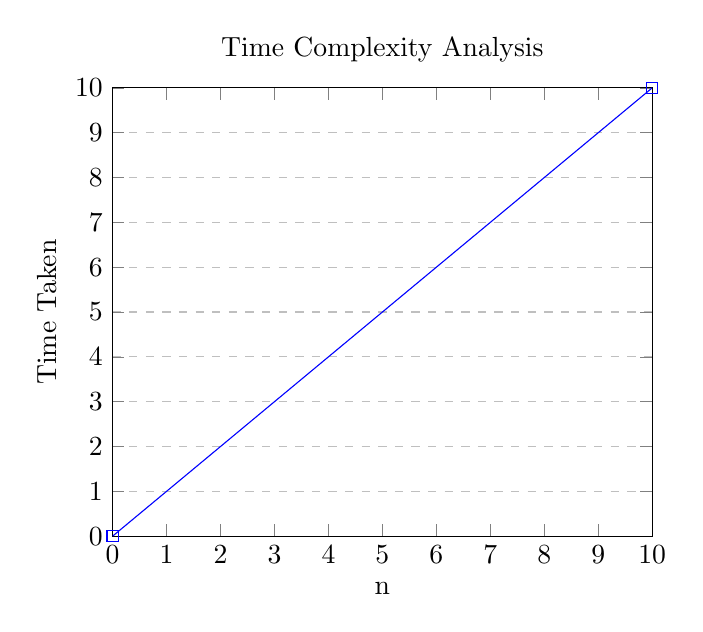
\begin{tikzpicture}
\begin{axis}[
    title={Time Complexity Analysis},
    xlabel={n},
    ylabel={Time Taken},
    xmin=0, xmax=10,
    ymin=0, ymax=10,
    xtick={0,1,2,3,4,5,6,7,8,9,10},
    ytick={0,1,2,3,4,5,6,7,8,9,10},
    legend pos=north west,
    ymajorgrids=true,
    grid style=dashed,
]

\addplot[
    color=blue,
    mark=square,
    ]
    coordinates {
    (0,0)(10,10)
    };
    
\end{axis}
\end{tikzpicture}

By the experimental analysis, we found that in  case of optimized approach, on increasing the number of numbers the graph is strictly increasing with a bend (or concavity) towards horizontal axis. Thus the overall time increases with an increase in size.

\paragraph{Space Analysis:}Following is the graph representing the space complexity of the algorithm.\\\\
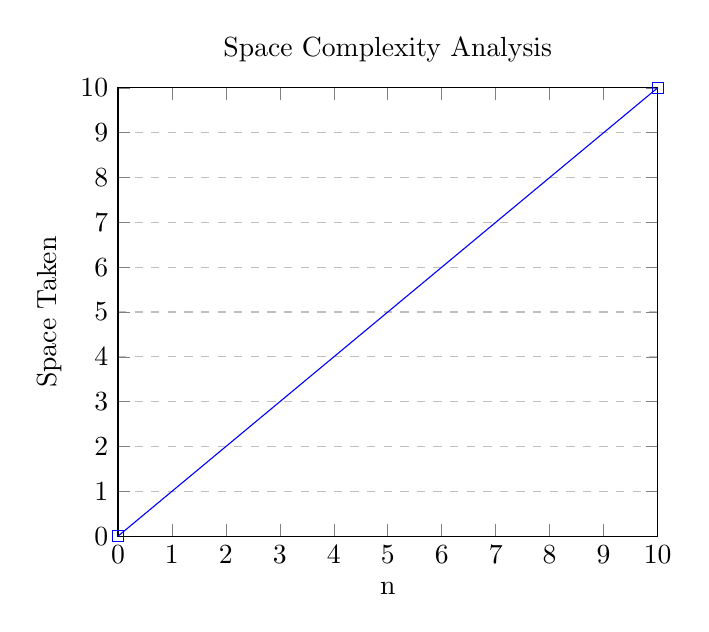
\begin{tikzpicture}
\begin{axis}[
    title={Space Complexity Analysis},
    xlabel={n},
    ylabel={Space Taken},
    xmin=0, xmax=10,
    ymin=0, ymax=10,
    xtick={0,1,2,3,4,5,6,7,8,9,10},
    ytick={0,1,2,3,4,5,6,7,8,9,10},
    legend pos=north west,
    ymajorgrids=true,
    grid style=dashed,
]

\addplot[
    color=blue,
    mark=square,
    ]
    coordinates {
    (0,0)(10,10)
    };
    
\end{axis}
\end{tikzpicture}

By the experimental analysis, we found that in case of optimized approach, on increasing the number of numbers the graph is strictly increasing. Thus the overall space increases with an increase in size.\\

\paragraph{APOSTERIORI ANALISIS:}
Aposteriori analysis of an algorithm means we per- form analysis of an algorithm only after running it on a system. It directly depends on the system and changes from system to system. So for the a aposteriori analysis of the algorithm,we have run our code on the compiler and get values of the time.
% \includegraphics[width=\columnwidth, height=6cm]{time_2.jpeg}\begin{center}\textbf{Figure 5:} Time Complexity Graph\end{center}
\section*{Experimental Analysis}
In the following table some cases are plotted for the algorithm on our local machine,
\begin{center}
 \begin{tabular}{||c | c||} 
 \hline
 n & Time Taken (in ms) \\ [0.5ex] 
 \hline\hline
 10 & 0.003 \\ 
 \hline
 100 & 0.0039 \\
 \hline
 1000 & 0.015 \\
 \hline
 5000 & 0.058 \\
 \hline
 10000 & 0.11 \\
 \hline
 50000 & 0.59 \\
 \hline
 100000 & 1.2 \\
 \hline
 1000000 & 12 \\ [1ex] 
 \hline
\end{tabular}
\end{center}

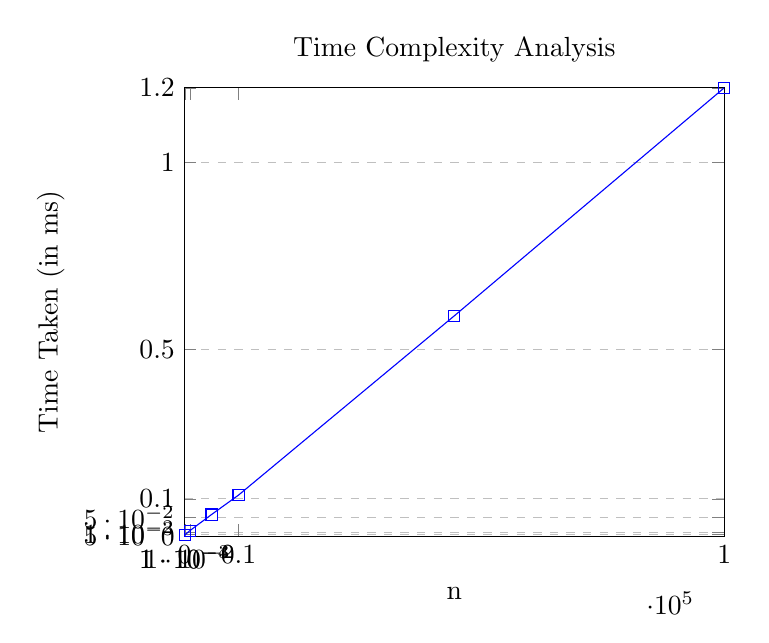
\begin{tikzpicture}
\begin{axis}[
    title={Time Complexity Analysis},
    xlabel={n},
    ylabel={Time Taken (in ms)},
    xmin=0, xmax=100000,
    ymin=0, ymax=1.2,
    xtick={0,10,100,1000,10000,100000,1000000},
    ytick={0,0.005, 0.01,0.05, 0.1,0.5,1,1.2},
    legend pos=north west,
    ymajorgrids=true,
    grid style=dashed,
]

\addplot[
    color=blue,
    mark=square,
    ]
    coordinates {
    (10,0.003)(100,0.0039)(1000,0.015)(5000,0.058)(10000,0.11)(50000,0.59)(100000,1.2)
    };
    
\end{axis}
\end{tikzpicture}

\section*{CONCLUSION}

So, with the above mentioned algorithms and their profiling, we come to the conclusion that this classical problem of finding the sum of n natural numbers is achieving its best time complexity of O(n) and space complexity of O(n).\\Also, when we are dealing with large numbers such as the one occupying 64-bits (long long integers), the complexity is same. So we can take the modulus of distance with 109+7 in order to make sure that it gets fit in the available data types(long long integer types more specifically).


\section*{REFERENCES}

\begin{enumerate}
\item Introduction to Divide and Conquer Technique:\\
https://www.geeksforgeeks.org/divide-and-conquer-algorithm-introduction/
\item Introduction to Algorithms by Cormen,Charles, Rivest and Stein.\\
https://web.ist.utl.pt/~fabio.ferreira/material/asa
\end{enumerate}\\

\section*{APPENDIX}
\textbf{To run the code, follow the following procedure:}
\begin{enumerate}
    \item Download the code(or project zip file) from the github repository.
    \item Extract the zip file downloaded above.
    \item Open the code with any IDE like Sublime Text, VS Code, Atom or some online compilers like GDB.
    \item Run the code following the proper running commands(vary from IDE to IDE)
    \begin{enumerate}
        \item \textbf{For VS Code:} Press Function+F6 key and provide the input on the terminal.
        \item \textbf{For Sublime Text:} Click on the Run button and provide the input.\\
    \end{enumerate}
\end{enumerate}
\textbf{Code for Implementation is:}
\lstset { %
    language=C++,
    backgroundcolor=\color{black!5},
    basicstyle=\footnotesize,
}

\begin{lstlisting}
#include<bits/stdc++.h>
using namespace std;

int sumArray(int Array[], int size){
    //base case
    if (size == 0)
        return 0;
    else if (size == 1)
        return Array[0];

    //divide and conquer
    int mid = size / 2;
    int rsize = size - mid;
    int lsum = sumArray(Array, mid);
    int rsum = sumArray(Array + mid, rsize);
    return lsum + rsum;
}

int main(){
    int n;
    cout<<"Enter a number : ";
    cin>>n;
    int arr[n];
    for(int i=1;i<=n;i++)
        arr[i-1]=i;
    cout<<"Sum will be:"<<sumArray(arr,n)<<endl;
}
\end{lstlisting}
\end{multicols*}
\clearpage

	
\end{document}